% Typischer Heimrouter von vorne (neutral, ohne Marke): Gehäuse, Antennen, Status-LEDs.
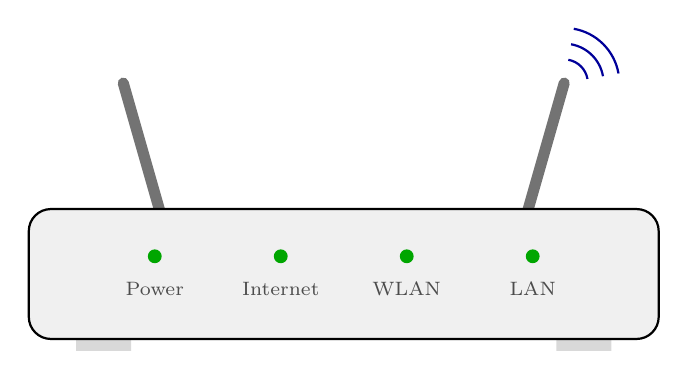
\begin{tikzpicture}[
        antenne/.style={line width=4pt, line cap=round, black!55},
        led/.style={circle, inner sep=0pt, minimum size=5pt, fill=green!65!black},
        ledtext/.style={font=\scriptsize, black!70, anchor=north}
    ]
    % Antennen hinter dem Gehäuse
    \draw[antenne] (-2.2,1.0) -- (-2.8,3.1);
    \draw[antenne] (2.2,1.0) -- (2.8,3.1);
    % Funkwellen
    \foreach \r in {0.3,0.5,0.7}
        \draw[blue!60!black, thick] (2.8,3.1) ++(10:\r) arc (10:80:\r);
    % Gehäuse
    \fill[black!15] (-3.4,-0.15) rectangle (-2.7,-0.3) (2.7,-0.15) rectangle (3.4,-0.3);
    \draw[thick, fill=black!6, rounded corners=8pt] (-4,-0.15) rectangle (4,1.5);
    % Status-LEDs
    \foreach \x/\t in {-2.4/Power, -0.8/Internet, 0.8/WLAN, 2.4/LAN} {
        \node[led] at (\x,0.9) {};
        \node[ledtext] at (\x,0.7) {\t};
    }
\end{tikzpicture}
